% @Author: Nizar TENZEKHTI
% @Date:   2019-08-08
\documentclass[12pt, oneside, a4paper]{enis-pfe-report}
\graphicspath{{./images/}}
%% TODO: Remove this function when done %%
%\newcommand\todoin[2][]{\todo[inline, caption={2do}, #1]{
%\begin{minipage}{\textwidth-4pt}#2\end{minipage}}}

%%%%%%%%%%%%%%%%%%%%%%%%%%%%%%%%%%%%%%%%%%%%%%%%%%%%%%%%%%%
% Include useful commands
%%%%%%%%%%%%%%%%%%%%%%%%%%%%%%%%%%%%%%%%%%%%%%%%%%%%%%%%%%%
\newcommand{\reportAuthor} {%
  Prénom \textsc{NOM}%
}

\newcommand{\reportTitle} {%
   TITRE DU PROJET \\ Title%
}

\newcommand{\reportSubject} {%
   TITRE DU PROJET \\ Title%
}

\newcommand{\dateSoutenance} {%
  jj/mm/aaaa%
}

\newcommand{\studyDepartment} {%
  Génie Systèmes Électroniques 
et Communication%
}

\newcommand{\ENIS} {%
  École nationale des ingénieurs de Sfax%
}

\newcommand{\codePFE} {% Reference %
}

\newcommand{\juryPresident} {%
  Mr Foulen \textsc{Fouleni}%
}
\newcommand{\juryPresidentDesc} {%
  President%
}

\newcommand{\juryMemberOne} {%
  Ms Foulena \textsc{Foulenia}%
}
\newcommand{\juryMemberOneDesc} {%
  Supervisor %Mentor
}

\newcommand{\juryMemberTwo} {%
  Mr Foulen \textsc{Fouleni}%
}
\newcommand{\juryMemberTwoDesc} {%
  Reviewer% Examiner, Reporter
}

\newcommand{\specialcell}[1]{%
  \begin{tabularx}{\textwidth}{@{}X@{}}#1\end{tabularx}%
}

%%%%%%%%%%%%%%%%%%%%%%%%%%%%%%%%%%%%%%%%%%%%%%%%%%%%%%%
% Add your own commands here
%%%%%%%%%%%%%%%%%%%%%%%%%%%%%%%%%%%%%%%%%%%%%%%%%%%%%%%
\newcommand{\MyCommand} {%
  Does nothing really%
}

\hypersetup{
  pdftitle={\reportTitle~-~\reportSubject},%
  pdfauthor={\reportAuthor},%
  pdfsubject={\reportSubject},%
  pdfkeywords={report} {internship} {pfe} {enis}
}
\dominitoc
\begin{document}
    \doublespacing{}% Double spacing between lines
    \pagenumbering{roman}% i ii iii iv ...
        \thispagestyle{empty}
\begin{titlepage}
\begin{center}
%%%%%%%%%%%%%%%%%%%%%%%%%%%%%%%%%%%%%%%%%%%%%%%
% THE HEADER
%%%%%%%%%%%%%%%%%%%%%%%%%%%%%%%%%%%%%%%%%%%%%%%
{%
  \fontsize{9pt}{9pt}\selectfont%
  \begin{tabularx}
  {\textwidth}
  { @{} p{0.35\textwidth} @{} p{0.02\textwidth} @{} p{0.3\textwidth} @{} p{0.02\textwidth} @{} p{0.35\textwidth} @{} }
    \centering%
Ministère de l'Enseignement supérieur
et de la Recherche scientifique\\%
Université De SFAX\\
المدرسة الوطنية لإلكترونيك والاتصالات بصفاقس
    \begin{spacing}{1}
    \end{spacing}
    \begin{spacing}{0.05}
    \noindent
    \end{spacing}
    \begin{spacing}{0.05}
    \noindent
    \\
    \end{spacing}
    &%
    % Column 2 is empty 
    &%
    % Column 3
    \centering%
    \multirow{2}{\linewidth}{%
      \centering%
      
\includegraphics[width=4cm, height=2cm]{images/enetcomlogo.png}%
    }%
    &%
    % Column 4 is empty 
    &%
    % Column 5
    \centering%
    \textbf{%
École nationale d'électronique et des télécommunications de Sfax\\
Département Télécommunications
    }%
    \tabularnewline%
    % Line 2
    \centering%
    %
    &%
    % Column 2 is empty 
    &%
    % Column 3 is empty (contains the ENETCOM logo)
    &%
    % Column 4 is empty 
    &%
    % Column 5
    \centering%
    \vspace{20pt}
    \textbf%
     %
    \tabularnewline%
    \arrayrulecolor{reportType}%
    \specialrule{0.75pt}{2pt}{0pt}%
    \specialrule{2.00pt}{1pt}{0pt}%
   \end{tabularx}
}


%%%%%%%%%%%%%%%%%%%%%%%%%%%%%%%%%%%%%%%%%%%%%%%
% THE PAGE CONTENT
%%%%%%%%%%%%%%%%%%%%%%%%%%%%%%%%%%%%%%%%%%%%%%%
\vspace{30pt}
{%
  \renewcommand*{\familydefault}{\defaultFont}
  \fontsize{34pt}{34pt}\selectfont%
  Rapport de stage d’ouvrier
}\\
\vspace{12pt} {%
  \fontsize{13pt}{13pt}\selectfont%
  \textbf{\textit{intitulé}}\\
}%
\vspace{12pt} {%
  \begin{spacing}{0.05}
    \rule{200pt}{2pt}\\
    \rule{200pt}{0.75pt}\\
  \end{spacing}
  \renewcommand*{\familydefault}{\defaultFont}
  \fontsize{17pt}{17pt}\selectfont%
  \vspace{20pt}
  \textbf{
Application web de montage et diffusion\\ du contenus vidéos
  \\%
  }
  \vspace{20pt}
  \begin{spacing}{0.05}
    \rule{200pt}{0.75pt}\\
    \rule{200pt}{2pt}\\
  \end{spacing}
}
\vspace{20pt}
\textbf{\textit{}}\\
\vspace{3pt} {%
  \fontsize{13pt}{13pt}\selectfont%
  \textbf{\textit{Réalisé par :}}\\
  \textbf{Ibn Hamda Eya}\\
  \textbf{Hammami Sahar}\\
  \textit{au sien de:}\\
    
\includegraphics{images/djagoralogo.png}
}%
\vspace{20pt} {%
\\
  \fontsize{15pt}{15pt}\selectfont%
  \textit{Sous la direction du :}\\
  \textbf{Mr Tarek OUNI}\\
  Année Universitaire : 2020/2021
}%
\vfill
\end{center}
\end{titlepage}
    \doublespacing{}
    \newpage
    \pagenumbering{arabic}
    \chapter*{\centering \textcolor{purple}{Remerciements}}
%\addstarredchapter{REMERCIEMENT}
%\addcontentsline{toc}{chapter}{REMERCIEMENT}
%\adjustmtc
\thispagestyle{MyStyle}
J’ai l’honneur d’exprimer mes sincères remerciements à toute l’équipe de la société Djagora.\par

Je tiens à remercier mon encadrent Ouni Tarak pour sa confiance et son soutien tout au long de ma période de stage.\par

J’adresse mes remerciements aussi aux personnels du département informatique pour leurs explications détaillés tout au long du déroulement du stage car c’est grâce à leurs supports et leurs engagements que j’ai pu achever ce travail.\par
    \renewcommand*\contentsname{\centering \textcolor{cyan}{TABLE DES MATIÈRES}}
        \addtocontents{toc}{\protect\thispagestyle{MyStyle}}
    \begin{spacing}{1}
    \tableofcontents
    \end{spacing}
    \addtocontents{lof}{\protect\thispagestyle{MyStyle}}
    \renewcommand{\listfigurename}{LISTE DES FIGURES}
    \addto\captionsenglish{
\renewcommand{\listtablename}{Tables}}
    \begin{spacing}{1}
    \end{spacing}
    \addcontentsline{toc}{chapter}{\listfigurename}
    \adjustmtc
    \chapter*{\centering \textcolor{cyan}{INTRODUCTION GÉNÉRALE}}
\markboth{\MakeUppercase{INTRODUCTION GÉNÉRALE}}{}
\renewcommand{\labelitemi}{$\bullet$}
%\addstarredchapter{INTRODUCTION GÉNÉRALES}
\addcontentsline{toc}{chapter}{INTRODUCTION GÉNÉRALE}
\adjustmtc
\thispagestyle{MyStyle}
Durant ces dernières années, l’informatique s’est imposée d’une manière très impressionnante dans les entreprises, cela est dû à son apport fructueux dans le domaine de gestion de base de données et pour assurer la bonne communication.\par

Aujourd’hui, vu l’intérêt croissant de vouloir gagner du temps, de communiquer mieux avec des moyens plus perfomante et plusieurs autres raisons, il a été question de chercher des solutions informatiques susceptibles de répondre aux besoins des utilisateurs.\par
C’est dans ce cadre que s’inscrit notre stage d’été qui consiste à réaliser une application «\textbf{Développement d’une application web de montage et diffusion du contenus vidéos}» .\par
au sein de la société Djagora. Cette application permet d’informatiser les différentes tâches relatives à la gestion et la diffusions des vidéos . Ce rapport sera réparti en 3 chapitres:\par 
\begin{itemize}
        \item Le premier chapitre, intitulé «\textbf{Présentation générale du projet}» est consacré à présenter l’environnement du projet et le cadre de sa réalisation.
    \item Le deuxième chapitre, intitulé «\textbf{spécifications des besoins} » présente la partie de spécifications des besoins de notre application .
    \item Le dernier chapitre, intitulé «\textbf{Réalisation} » présente l’architecture technique de l’application et les interfaces.
\end{itemize}

    \chapter{\begin{center}
    \textcolor{purple}{Présentation générale du projet}
\end{center}}
\section*{\textcolor{cyan}{Introduction}}
L’étude de projet est une démarche stratégique visant à organiser le bon déroulement d’un projet et d’assurer la conduite de toutes les phases qui le constituent.\par
Une étude complète et efficace conduit généralement à la réussite d’un projet. Cette étude fera donc l’objet de notre premier chapitre qui sera consacré à la présentation de l’organisme d’accueil, et la présentation du projet.\par
\section{\textcolor{cyan}{Présentation de l’organisme d’accueil :}}
Djagora Fablab est le 6éme fablab issu d'un partenariat entre la \textbf{Fondation Orange} et La \textbf{Fondation Djagora}.\par
Situé à la Technopole de Sfax, au village de l'entrepreneuriat, Djagora Fablab intervient dans la chaine de valeur de création de start-up et de l'innovation, coté formation et prototypage.\par
Djagora Fablab est un ouvert au public mettant à la disposition de ses utilisateurs les ressources techniques, technologiques et humaines nécessaires à la conception, l’optimisation, la réparation de toute sorte d’objets.\par
Le Fablab dispose d'une large gamme d'outils de fabrication, notamment une découpeuse laser, une fraiseuse numérique, une imprimantes 3D, un Workstation Pro, etc...
\par
\begin{center}
    
\includegraphics[width=5cm]{images/djagora2.png}
    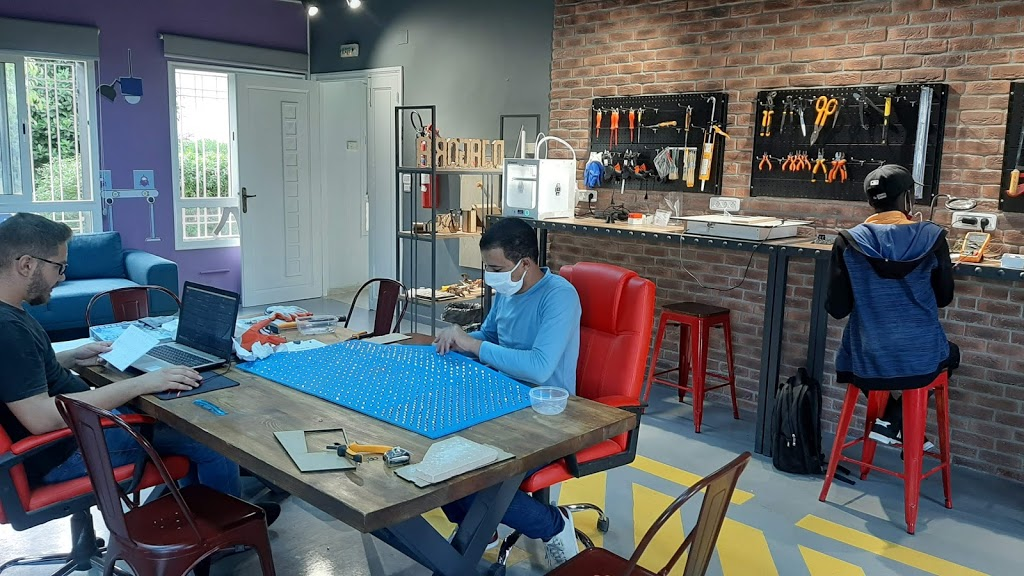
\includegraphics[width=10cm]{images/djagoraImage.png}
    \caption{\textbf{Djagora}}
    \label{fig:my_label}\\
\end{center}
\textbf{\textcolor{cyan}{Djagora Academy:}}\par
Djagora Academy est un programme a pour but d’accélérer l’employabilité des jeunes de l’enseignement supérieur. Il s’adresse essentiellement aux étudiants jeunes diplômés ou en fin de cycle Licence, Master ou Ecole d’Ingénieur.\par
Le programme Djagora Academy repose sur 3 piliers essentiels:\par
\begin{itemize}
    \item Le savoir-être
    \item Le savoir-faire
    \item La réalisation de prototype
\end{itemize}\par
\begin{center}
    
\includegraphics[width=5cm]{images/djagoraAcademy.png}\\
\end{center}
Sur une durée de 5 à 6 mois les étudiants vont developper l’ensemble des compétences recherchées par les employeurs en mettant en pratique toutes les connaissances théoriques apprises au cours de leur cursus académique.\par
Chaque étudiant aura l’opportunité de mettre en pratique ses compétences en “critical thinking” par la conception et la formalisation écrite d’un problème réel en projet, la mobilisation de l’ensemble des parties prenantes grâce à la formation Leadership, la communication au tour du projet grâce à la formation en Digital Marketing, le management de projet grâce à l’outil SCRUM Agile, le travail en équipe grâce au Leadership immersion camp lors de la semaine d’intégration. Enfin, l’approche entrepreneurial grâce a la participation aux compétitions pour startup et salons. Les étudiants ayant participés au programme bénéficient de certifications professionnelles telles que le Six Sigma, le Digital Marketing et SCRUM Agile reconnues au niveau internationale. Nos étudiants se démarquent par le fait d’avoir eu l’opportunité d’appliquer l’ensemble des outils relatifs à ces certifications professionnelles dans des projets réels et ce dans un environnement qui encourage la prise de risque. Le rôle des mentors reste clé dans la réalisation de ce programme.\par
\section{\textcolor{cyan}{Présentation du projet:}}
\subsection{Problème :}
D’un côté, des plateformes de contenus de plus en plus complexes. De l’autre, des publics difficiles à capter, sur-sollicités…\par
Dans ce contexte, la vidéo online est l’un des rares médias qui rende l’information intelligible, attractive, qui valorise les individus, encourage la participation et le dialogue.\par
La WebTV nous est apparue comme étant la scénarisation la plus efficace des contenus vidéo.\par
\subsection{Technologies utilisées:}
\textbf{Node.js} est une plateforme logicielle libre en JavaScript, orientée vers les applications réseau évènementielles hautement concurrentes qui doivent pouvoir monter en charge.
\textbf{Express.js} est un framework pour construire des applications web basées sur Node.js. C'est de fait le framework standard pour le développement de serveur en Node.js.\par
La figure 2 représente les logos de Node.js et Express.js.\par
\begin{center}

\includegraphics[width=5cm]{images/nodeexpress.png}
     \caption{logos de Node.js et Express.js}
     \label{fig:my_label}\\
\end{center}
\subsubsection{\textbf{Node.js Express VS PHP:}}
Les frameworks PHP modernes améliorent beaucoup leur qualité de code, mais ces frameworks sont encore très en retard par rapport à Node.js en termes de fonctionnalités et de productivité.\par
 PHP est verbeux, peu flexible, et difficile à débogguer. Parce qu'il est conçu pour sa facilité d'utilisation plutôt que pour la qualité du code, il est trop facile d'écrire du code insécure (présentant des failles de sécurité) ou du code spaghetti.\par
\subsubsection{\textbf{Architecture MVC}}[hb]
MVC(Figure2) est un patron de conception(Design Pattern) très répandu pour réaliser la structure des sites web. Ce patron de conception est une solution éprouvée et reconnue permettant de séparer l’affichage des informations, les actions de l’utilisateur et l’accès aux données.En effet, il permet de faciliter le dialogue l’utilisateur et le serveur d’application et d’augmenter les performances de l’application.\par
 Ce modèle comporte trois types de module:\par
 \begin{itemize}
     \item Un modèle (Model) faite grace NodeJS Express.
     \item Une vue (View) contient les pages (CSS+HTML+ JS).
     \item Un contrôleur (Controller) contient les scripts JS qui permet la logique concernant les actions effectuées par l'utilisateur.
 \end{itemize}
 \begin{figure}[hb]
     \centering
     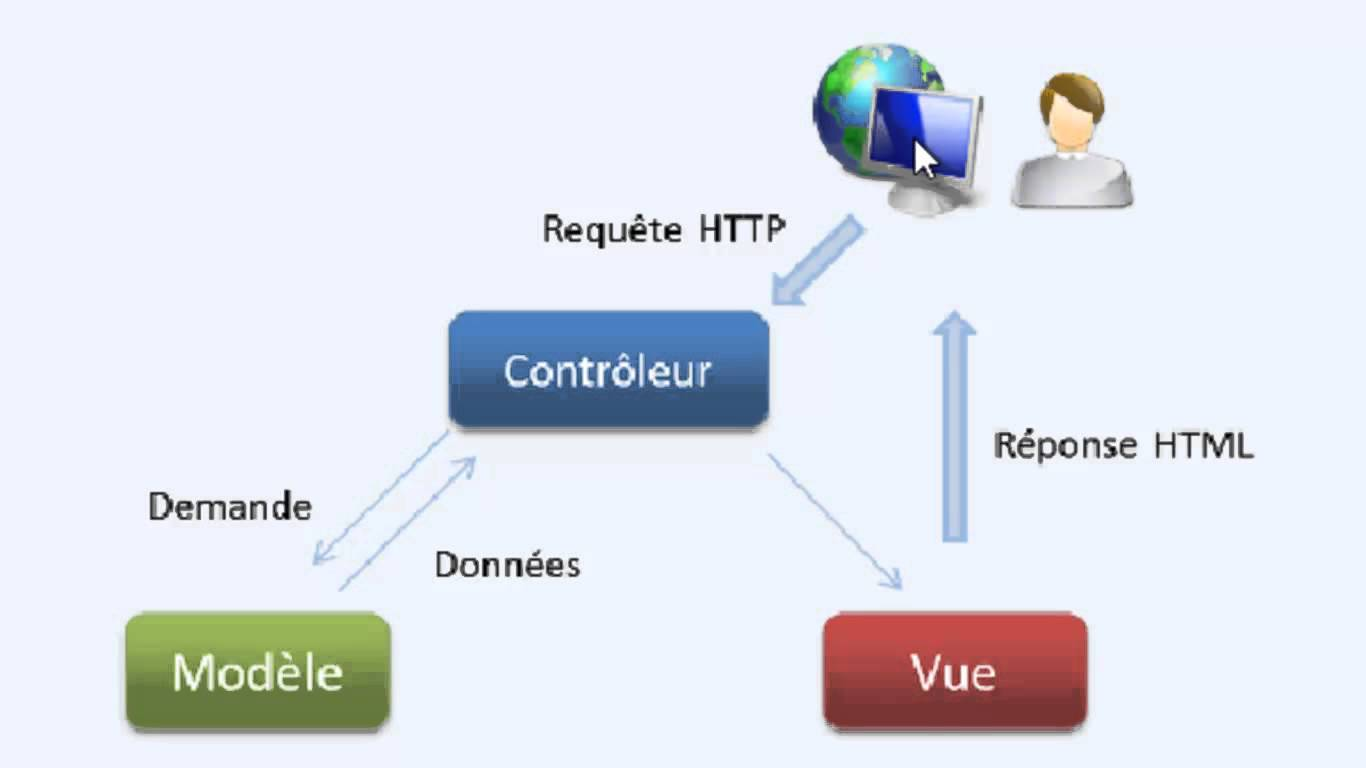
\includegraphics[width=10cm]{images/mvc.png}
     \caption{Architecture MVC}
     \label{fig:my_label}
 \end{figure}
    \chapter{\textcolor{purple}{Chapitre 2 : Spécification des besoins & Réalisation}}
\section{\textcolor{cyan}{Spécification des besoins:}}
\subsection{Besoin spécifié:}
Dans le domaine de web la communication entre les utilisateurs devient une nécessité, et le communication vidéo et audio a une interactivité mieux que les messages, donc Djagora veut une plateforme de communication sécurisé qui permet à ses employées de se connecter dans un space privé sans utiliser les plateformes comme Google meet ou discord et mettre des réunions dans des room de chat.\par
Lorsque l’utilisateur fait un login il peut joindre un room qui est identifié par un code, ce code est nécessaire pour entrer ou sortir de room.\par
Ce plateforme est un plateforme web, notre tâche se présente dans l’authentication le développement de login et sign up avec le chat vidéo ou audio seulement.\par
Dans ce cas, on a utilisé l’API de WEBRTC qui va assurer la communication entre les différents employées de la même room.\par
\subsection{Webrtc:}
C’est quoi webrtc?\newline
Il permet d’ajouter des capacités de communication en temps réel à l’application qui fonctionne sur la base d'une norme ouverte. Elle prend en charge la vidéo, la voix et les données génériques à envoyer entre pairs, ce qui permet aux développeurs de créer de puissantes solutions de communication vocale et vidéo.\par
La technologie est disponible sur tous les navigateurs modernes ainsi que sur des clients natifs pour toutes les principales plateformes. Les technologies qui sous-tendent le Webrtc sont mises en œuvre en tant que norme Web ouverte et disponibles sous forme d'API JavaScript ordinaires dans tous les principaux navigateurs. Pour les clients natifs, comme les applications Android et iOS, il existe une bibliothèque qui offre la même fonctionnalité. Le projet Webrtc est open-source et soutenu par Apple, Google, Microsoft et Mozilla, entre autres.\par
\section{\textcolor{cyan}{Réalisation :}}
\subsection{\textcolor{cyan}{Les technologies utilisées : Node.js et express:}}
\begin{enumerate}[label=(\alph*)]
    \item \textbf{node:}\\
    Node (ou plus formellement Node.js) est un environnement d'exécution open-source et multiplateforme qui permet aux développeurs de créer toutes sortes d'outils et d'applications côté serveur en JavaScript. Le moteur d'exécution est destiné à être utilisé en dehors du contexte d'un navigateur (c'est-à-dire en s'exécutant directement sur un ordinateur ou un système d'exploitation serveur). En tant que tel, l'environnement omet les API JavaScript spécifiques au navigateur et ajoute la prise en charge d'API de système d'exploitation plus traditionnelles, notamment HTTP et les bibliothèques de système de fichiers.\par
Du point de vue du développement d'un serveur web, Node présente un certain nombre d'avantages :\par
\begin{itemize}
    \item Excellentes performances ! Node a été conçu pour optimiser le débit et l'évolutivité des applications Web et constitue une bonne solution pour de nombreux problèmes courants de développement Web (par exemple, les applications Web en temps réel).\par
    \item Le code est écrit en "plain old JavaScript", ce qui signifie que moins de temps est passé à gérer le "changement de contexte" entre les langages lorsque vous écrivez du code côté client et côté serveur.\par
    \item JavaScript est un langage de programmation relativement nouveau et bénéficie d'améliorations dans la conception du langage par rapport à d'autres langages traditionnels de serveur Web (par exemple, Python, PHP, etc.). De nombreux autres langages nouveaux et populaires se compilent/se convertissent en JavaScript, de sorte que vous pouvez également utiliser TypeScript, CoffeeScript, ClojureScript, Scala, LiveScript, etc.\par
    \item Le gestionnaire de paquets node (NPM) donne accès à des centaines de milliers de paquets réutilisables. Il dispose également de la meilleure résolution de dépendances de sa catégorie et peut être utilisé pour automatiser la majeure partie de la chaîne d'outils de construction.\par
    \item Node.js est portable. Il est disponible sur Microsoft Windows, macOS, Linux, Solaris, FreeBSD, OpenBSD, WebOS et NonStop OS. En outre, il est bien supporté par de nombreux fournisseurs d'hébergement web, qui fournissent souvent une infrastructure et une documentation spécifiques pour l'hébergement de sites Node.\par
\end{itemize}
\item \textbf{Express:}\\
Express est le Framework web Node le plus populaire, et est la bibliothèque sous-jacente pour un certain nombre d'autres Framework web Node populaires. Il fournit des mécanismes pour :\par
\begin{itemize}
    \item Écrire des gestionnaires pour les demandes avec différents requêtes HTTP à différents chemins URL (routes).
    \item Intégrer des moteurs de rendu de type "vue" afin de générer des réponses en insérant des données dans des modèles.\par
    \item Définissez les paramètres courants des applications Web, comme le port à utiliser pour la connexion et l'emplacement des modèles utilisés pour le rendu de la réponse.\par
    \item Ajouter un middleware supplémentaire de traitement des demandes à n'importe quel point du pipeline de traitement des demandes.
\end{itemize}
Bien qu'Express soit en soi assez minimaliste, les développeurs ont créé des paquets de middleware compatibles pour répondre à presque tous les problèmes de développement Web. \par
Il existe des bibliothèques 	permettant de travailler avec les cookies, les sessions, les connexions 	d'utilisateurs, les paramètres d'URL, les données POST, les en-têtes de sécurité, et bien d'autres encore. Vous trouverez une liste des paquets de middleware maintenus par l'équipe Express à l'adresse Express 	Middleware (ainsi qu'une liste de certains paquets tiers populaires).\par
\end{enumerate}
\subsection{\textcolor{cyan}{Les interfaces}}
    \centering
    
\includegraphics[width=12cm]{images/indexPage.png}\\
C’est la page d’accueil de notre application, il y a 3 boutons chacun d’entre eux comporte comme un lien.\par
    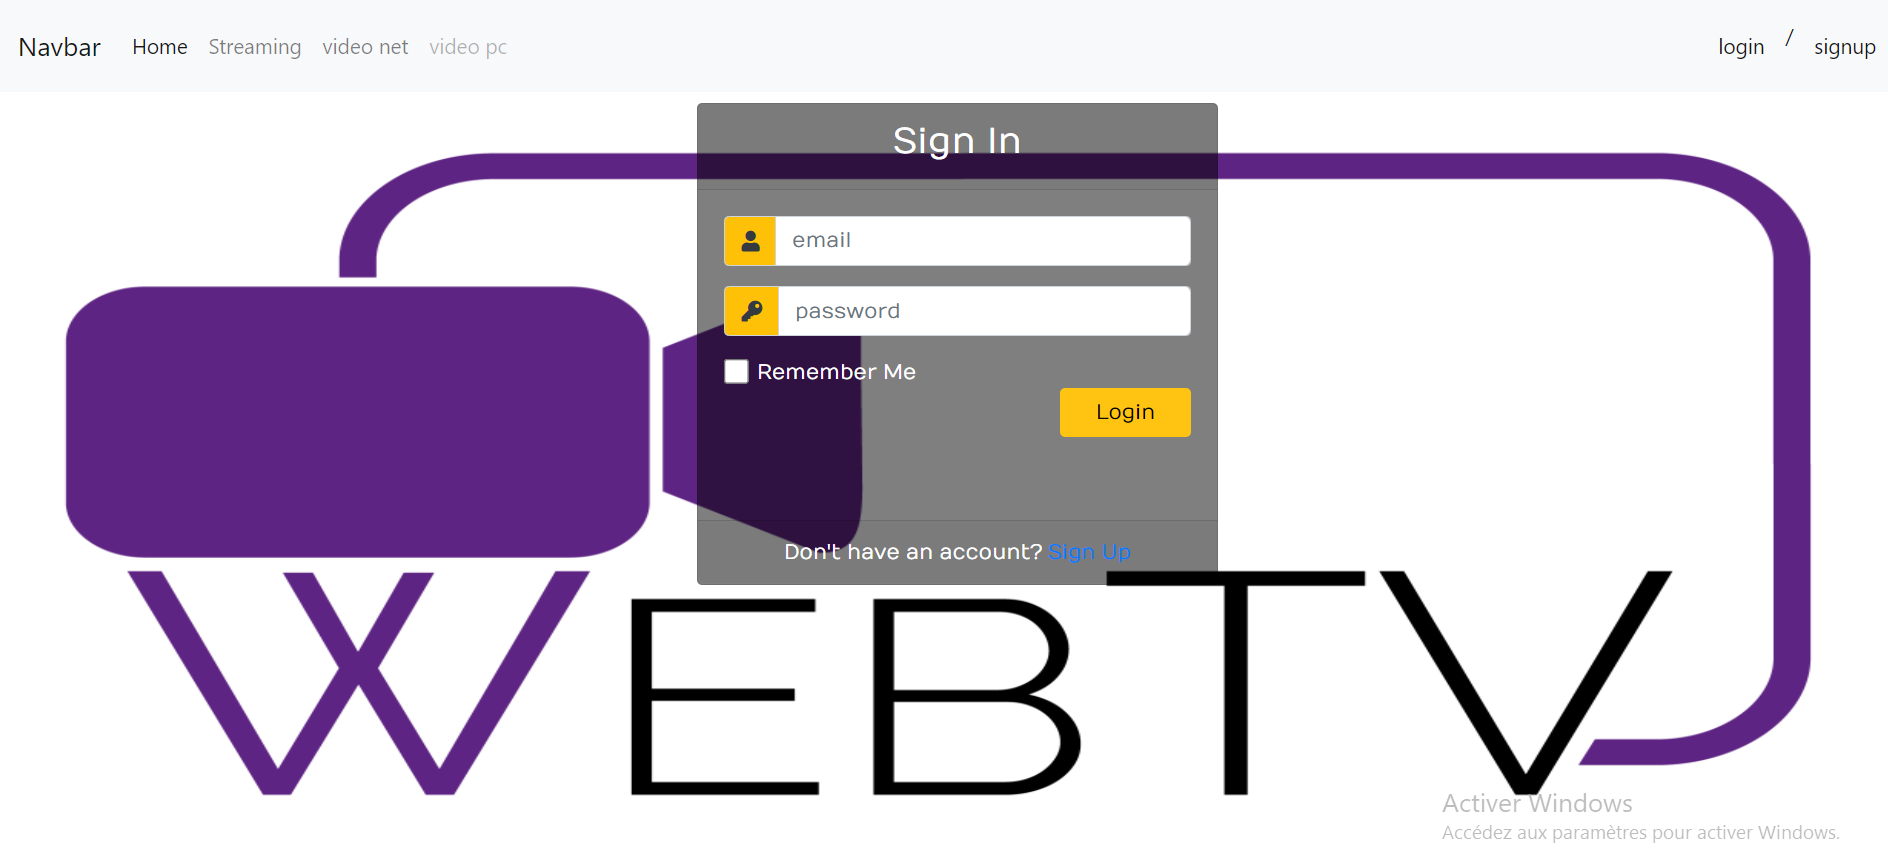
\includegraphics[width=12cm]{images/authentificationPage.png}\\
    C’est la page d’authentification des utilisateurs en entrant l’ email et le mots de passe pour ouvrir une session.\par
    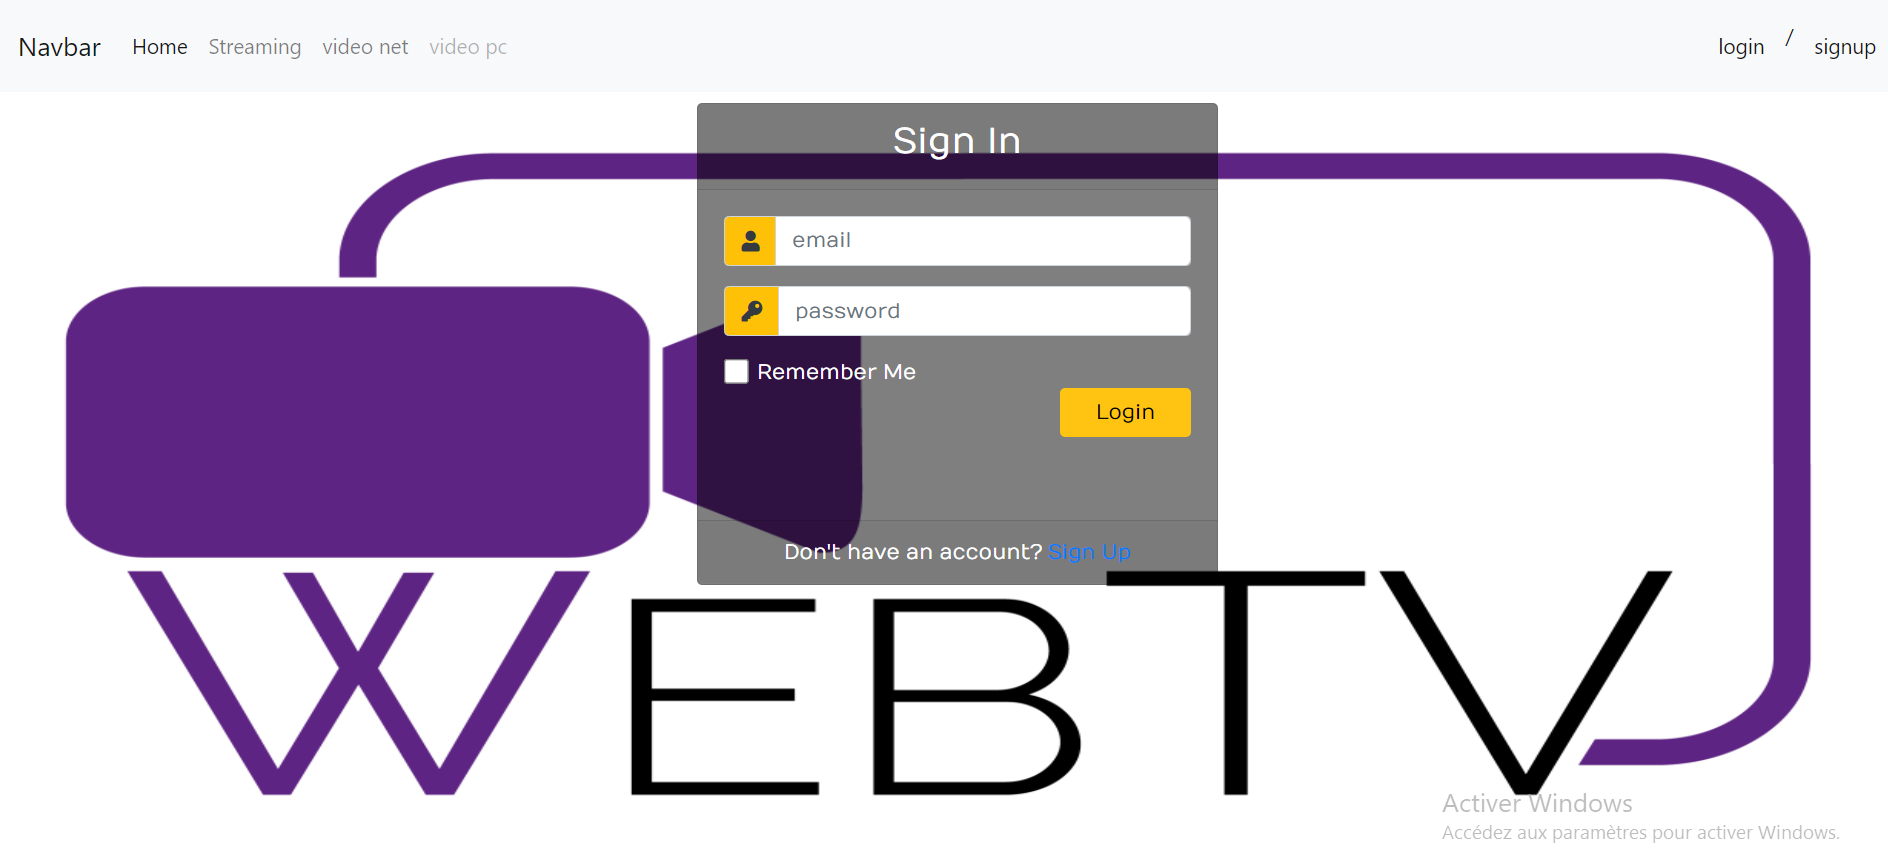
\includegraphics[width=12cm]{images/authentificationPage.png}\\
    En cliquant sur le bouton «video net », un vidéo va s’ouvrit sur la page.\par
    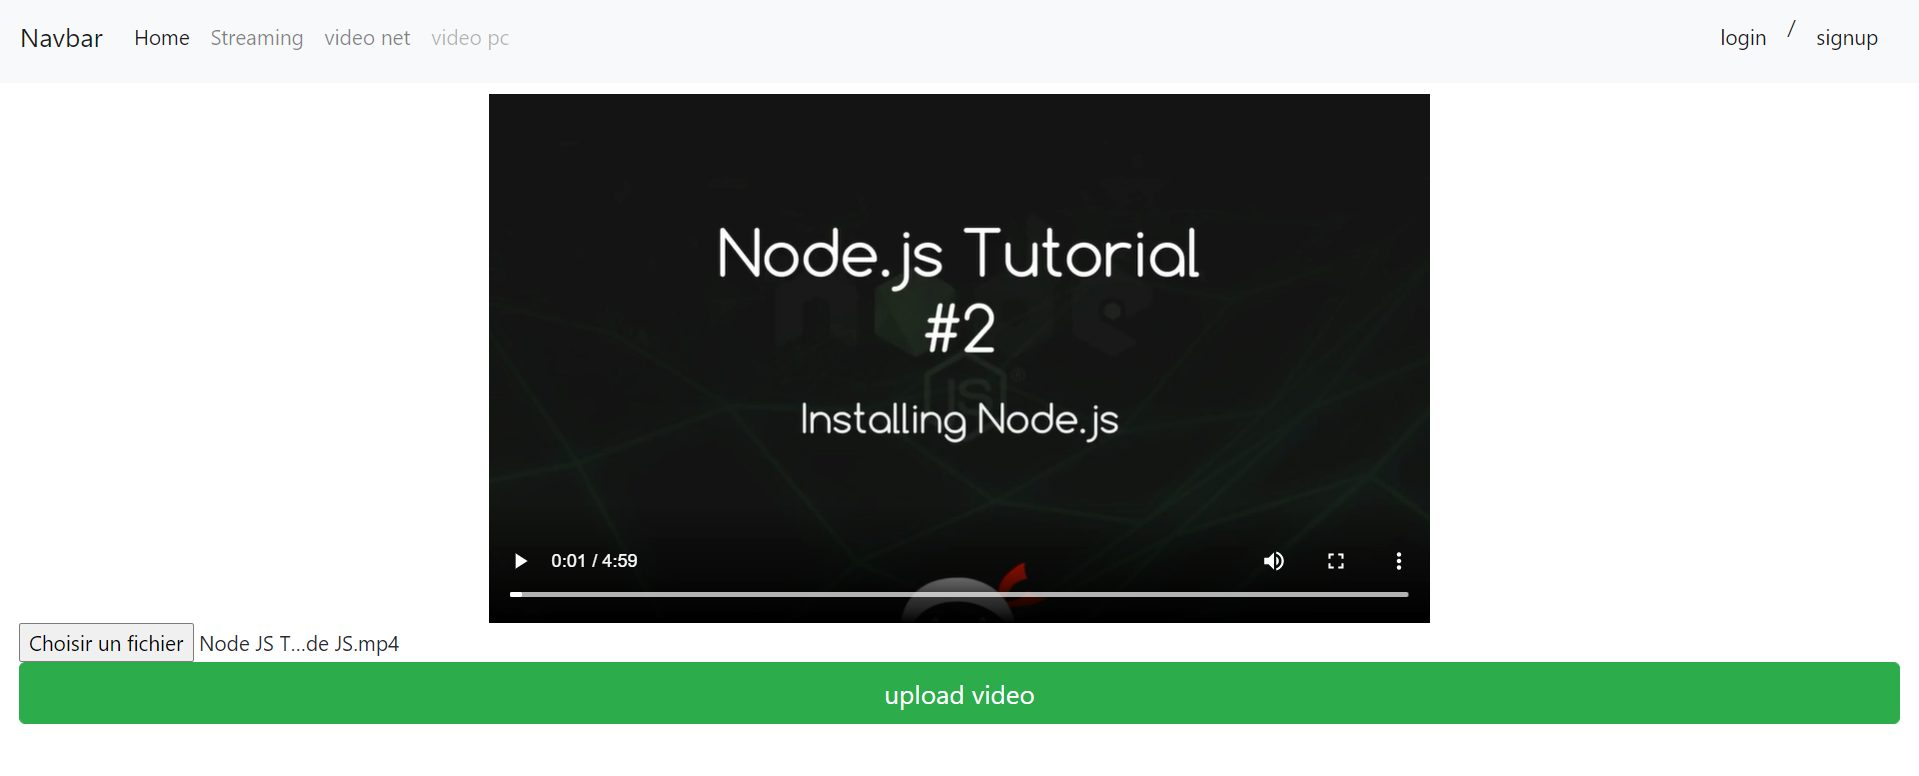
\includegraphics[width=15cm]{images/videoPc2.png}\\
    En cliquant sur le bouton « Choisir un fichier » , un dialogue s’ouvrit qui n’accepte que les fichiers vidéo et en choisissant un vidéo enregistré dans le pc, la page va s’ouvrit le vidéo choisi.\par
    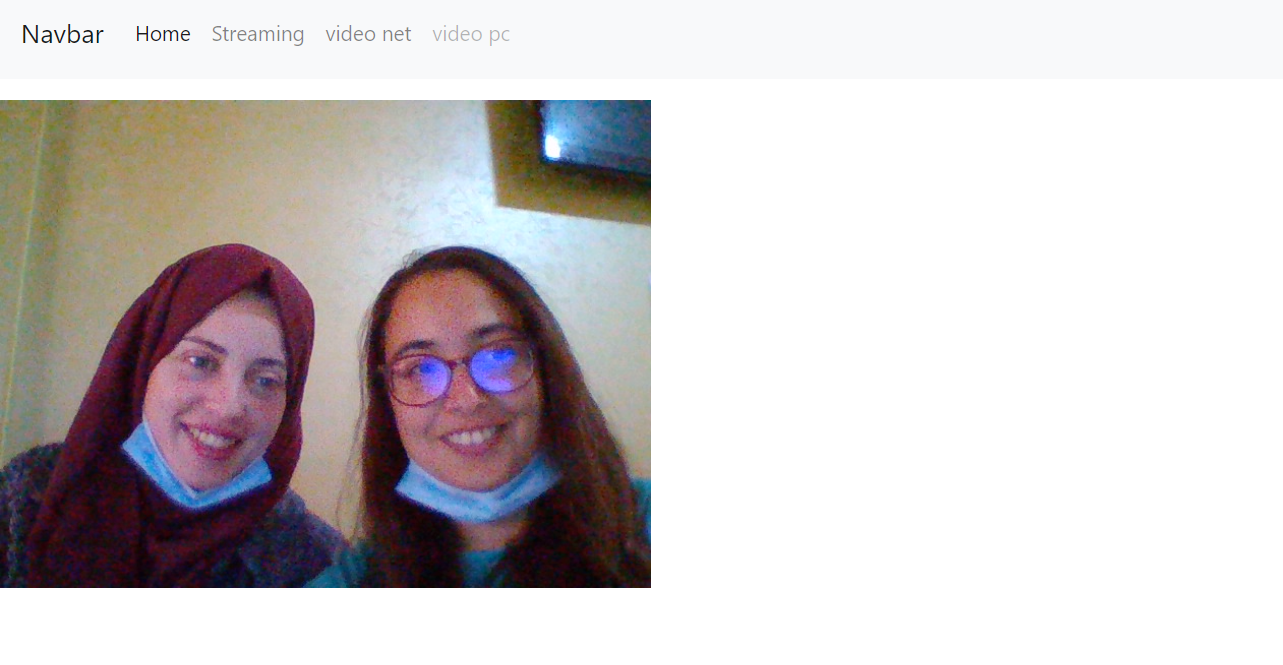
\includegraphics[width=15cm]{images/streaming.png}\\
    En cliquant sur le bouton « Streaming », cette page va s’ouvrit contenant une demande d’ouvrir le Cam et l’audio. En acceptant une entre eux, l’utilisateur va joindre le room .\par

\subsection{\textcolor{cyan}{deploiement heroku}}
Heroku est un PaaS (Platform as a Service) destinée au développement dans le Cloud. Heroku prend en charge les langages Ruby on Rails, Java, JavaScript, Node.js, Python, Scala et Clojure.\par
\subsection{\textcolor{cyan}{lien du travail}}
\hyperlink{https://webapprtcsahareya.herokuapp.com/}{\textcolor{red}{https://webapprtcsahareya.herokuapp.com/}}\\

\includegraphics[width=15cm]{images/heroku.png}\\
\end{document}
